\documentclass{article}
\usepackage{fullpage}
\usepackage{amsmath,amssymb,amsthm,bm,enumerate,mathtools}
\usepackage[hidelinks]{hyperref}
\usepackage{natbib}
\usepackage{xcolor}
\usepackage{graphics}

\newcommand{\E}{\mathbb{E}}
\renewcommand{\P}{\mathbb{P}}
\newcommand{\mL}{\mathcal{L}}
\newcommand{\ip}[2]{\left\langle #1, #2 \right\rangle}
\newcommand{\ie}{\textit{i.e.,}\,}
\newcommand{\eg}{\textit{e.g.,}\,}
\newcommand{\nb}{\textit{n.b.,}\, }
\newcommand{\defn}{:=}

\newcommand{\comment}[1]{{\color{blue} \it #1}}

\newtheorem{thm}{Theorem}
\newtheorem{lem}{Lemma}
\newtheorem{prop}{Proposition}
\newtheorem{cor}{Corollary}
\theoremstyle{remark} 
	\newtheorem{rem}{Remark}
	\newtheorem{assn}{Assumption}
\theoremstyle{definition} 
	\newtheorem{mydef}{Definition} 
	\newtheorem{exmp}{Example} 
	\newtheorem{cond}{Condition}
	\newtheorem{conj}{Conjecture}


\begin{document}

% 1. *Intro*: Motivation about how many results about quant gen and methods assume Gaussian distributions.
%     Mention Levy walk macroevolution papers.
%     Point out that usual quant gen has *no* sweeps, while stable distributions would have sweeps (since some s would be bigger than 1/N).
%     Motivate with mixture model of effect sizes.
%     If stable distributions are a better model, what does that tell us? We can better understand the *noise* in evolution, i.e., predictability and saltation-ness.
%     (PETER)
% 
% 2. Motivation: empirical SNPs distributions in real data (PETER)
% 
% 3. Introducing infinitesimal model (in this case) (TODD)
% 
% 4. Proof following BEV in stable case (TODD)
% 
% 5. Theoretical results on stationary distributions (TODD)
% 
% 6. Simulations (PETER)

\title{\large{\bf
    Quantitative genetics with stable laws
}}

\author{ \begin{small}
    Todd Parsons \&
    Peter Ralph
\end{small}}

\date{\today}
\maketitle

\begin{abstract}
\end{abstract}

%%%%%%%%%%%%%%%%%%%%%%
\section{Introduction}

Much of the work to give a quantitative understanding to the observation that
offspring of sexual organisms resemble their parent,
has focused on \emph{quantitative genetics},
which is interestingly intermediate between a mechanistic model of genetics
and a purely phenomenological model.
The action of natural selection on genetic variants in the absence of genetic variation
is relatively well-understood (cite ewens),
but tractable mathematical models of evolution for recombining species
are elusive,
at least with some results of when the model might be a good description of reality.
For instance, a great deal of conceptual understanding and even quantitative predictions
have been made assuming that the distribution of trait values in a population is Gaussian
(cite Lande etcetera)
despite the absence of a plausible model that would make this true (cite turelli and barton).
One of the oldest and most concrete models of heritable trait evolution is the \emph{infinitesimal model}
which assumes a simple, explicit form for how an offspring's trait is inherited from their parents':
it is Normally distributed, with mean equal to the average of the parents' values.
Despite the inherent plausibility of this model,
(thanks to the Central Limit Theorem),
it was not until \citet{barton2017infinitesimal} that conditions under which this would be a good approximation
were made explicit,
through a formal convergence proof.

As suggested by its name, under the infinitesimal model the effects of any given genetic variant on the trait
is small (indeed, vanishing),
and so selection-driven trait shifts are mediated by small changes in frequencies of many alleles of small effect.
However, empirical understanding of the genetic basis of trait variation in real-world species
often finds a significant portion of heritable variation explained by variants at only a few loci.
There are many possible explanations for this observation,
including selection/publication bias,
filters for larger-effect variants due to spatially varying selection (cite),
ond/or grouping together of concordant alleles by linkage or inversions (cite).
However, it seems clear that in at least those cases where we understand the underlying molecular mechanisms
that mutations of large effect can be important in practice
(cite examples: insecticide resistance, coloration, etc),
and the consensus in the field is that traits exist on a spectrum between monogenic and polygenic,
and that many - if not most - are firmly in the intermediate, ``oligogenic'' region (cite),
where heritable trait variation is due both to segregating large- and small-effect variants.
Indeed, some sensible verbal models of the biological mechanisms by which a genetic change
comes to have an effect on an organism's trait
describe a hierarchy or range of ``proximities'' to the trait,
by which changes to more ``nearby'' genes have the possibility of causing larger changes in the trait
(cite omnigenic and others).
This suggests a mixture model for the effect size distribution:
perhaps the distribution of effect sizes within each gene is Normal,
but with a standard deviation that varies with ``proximity'' to the trait;
such mixtures can easily have large proportions of extreme values.

The infinitesimal model gains a great deal of generality by appealing to the Central Limit Theorem:
as shown by \citet{barton2017infinitesimal},
the distribution of segregation noise will be Normal, regardless of most of the details,
thanks to the universality of adding up a great many very small and independent things.
However, as is well known to probabilists,
there is a wider class of Central Limit Theorems,
which describe the distributions of sums of a great many independent and exchangeable things:
the \emph{stable laws}.
Roughly speaking, these say that if we add together $n$ independent copies of a random variable $X$
for which $\P\{ X > t \} \propto t^{-\alpha}$ for some $0 < \alpha < 2$,
then -- almost regardless of the details -- the result, scaled by $n^{1/\alpha}$,
is well-approximated by a universal form, the $\alpha$-stable distribution (and becomes exact, as $n \to \infty$).
In such ensembles, sinle large entries are important:
concretely, the largest of the $n$ copies will be of order $n^{1/\alpha}$,
so that e.g., for $\alpha=1$ a positive proportion of the sum of $n$ entries will be contributed by a single one.

This suggests exploring whether stable distributions might reasonably stand in for the Normal
in the infinitesimal model.
In this paper, we make rather preliminary explorations in that direction:
Does the universality shown by \citet{barton2017infinitesimal}
carry over when the distribution of effect sizes falls in the domain of attraction of a stable law?
What can be said about equilibrium trait distributions in this case?
And, is there any biological evidence that this theory might be relevant?

Stable distributions are by no means new to population biology.
For instance, it is a long-standing question how often the motions of organisms
are better modeled by essentially Brownian random walks or by L\'evy processes (cite),
and a growing literature studies the effects of such ``fat-tailed'' distributions
on the shapes and dynamics of traveling waves such as biological invasions (cite).
\comment{Other examples?}
More directly analogous to the problem we study here, \citet{landis2012phylogenetic}
found that an $\alpha$-stable process (with $\alpha \approx 1.5$) fit the evolution of log endocranial volume
on the primate phylogeny
better than either a Brownian model.
\comment{more}

\comment{TODO expand, put somewhere:}
There are several justifications for why a ``stable infinitesimal model'' might be useful:
(1) as a phenomenological model;
(2) if it matches empirical observations; or
(3) if there is a central limit theorem suggesting it would be a good approximation in a wide range of situations.

\subsection*{Orphaned text}
The ways in which genetic variants combine to determine an organisms' trait can be complex,
and epistatic interactions between alleles and between loci can be important in practice.
However, the question is sufficiently complex in the purely additive case
that a trait can be decomposed into a sum across loci of the contributions of the alleles from each locus.
Under this additive assumption it makes sense to discuss the ``effect size distribution'',
i.e., the distribution of how much alleles affect the trait value.

An offspring's trait differs from their parents for many reasons,
often most importantly because of differences in the environment in which they live.
The focus of quantitative genetics is on the contribution of heritable material to this variation:
the offspring's genetic material 


\comment{Will need this notation below:}
We focus on the \emph{infinitesimal model},
as described by \citet{barton2017infinitesimal},
which supposes that the trait value of an offspring
is equal to the average of their parents' trait values,
plus independent Gaussian noise with fixed variance,
\begin{equation} \label{eqn:offspring_model}
    X_o = \frac{X_m + X_f}{2} + \epsilon,
\end{equation}
where $\epsilon$, the ``segregation noise'',
is Gaussian with mean zero and variance $V_0$.
\comment{should call this something besides $\epsilon$}

%%%%%%%%%%%%%%%%%%%%%%
\section{Empirical observations}

It is mathematically intriguing to speculate what effect a non-Gaussian distribution
for $\epsilon$ would have on the dynamics induced by~\eqref{eqn:offspring_model}.
But, is there any evidence that non-Gaussian segregation noise is important in practice?
In this paper we focus primarily on the theory,
but first take a brief and imperfect look at what some data have to say on the topic.
To do this, we downloaded the GWAS results provided by~\citet{biobankSNPs}
for 7,221 phenotypes from 361,194 individuals from the March 2018 release of the UK Biobank.
After filtering (see details below) we were left with 695 binary illness-related phenotypes.
Taken at face value, these provide for each phenotype a set of estimates of the additive effect
of the alternative allele at a set of SNPs on the phenotype relative to the reference allele.
The phenotypes we consider were all binary and coded as 0/1,
so estimates could be thought of as additive adjustments to the risk
(i.e., effects are \emph{not} on a logit scale).
These estimates were obtained as the coefficient for the SNP in a simple linear model
fit to each phenotype for each SNP,
with the first 20 principal components and all combinations of age, age squared, and inferred sex as covariates;
we considered effects of those SNPs with a reported $p$-value less than $10^{-8}$.
There are a great many possible issues with these data;
however, the results seem consistent across many SNPs and phenotypes,
and we know of no reason that possible methodological artifacts
(e.g., confounding by uncorrected variables)
would specifically affect the decay of the tail of effect sizes.

Suppose that the phenotype of each individual is additive:
the maternal trait value is $x = \sum_i x_{i,1} + x_{i,2}$
and the paternal trait value is $y = \sum_i y_{i,1} + y_{i,2}$,
where $x_{i,1}$ and $x_{i,2}$ are the effects of the alleles carried
by the mother on each of the two chromosomes
at the $i^\text{th}$ locus, respectively.
Then the offspring's trait is $z = \sum_i z_{i,m} + z_{i,p}$,
where $z_{i,m} = \theta_{i,m} x_{i,1} + (1-\theta_{i,m}) x_{i,2}$,
and $\theta_{i,m} = 1$ with probability 1/2 and $\theta_{i,m} = 0$ otherwise;
and likewise $z_{i,p} = \theta_{i,p} y_{i,1} + (1-\theta_{i,p}) y_{i,2}$.
With this notation, the segregation noise $z - \frac{x+y}{2}$
is a sum of terms of the form
$$
    \left( \theta_{i,m} - 1/2 \right) x_{i,1}
    + \left( 1/2 - \theta_{i,m} \right) x_{i,2} 
$$
(and similar terms with $y$ in place of $x$).
Now let $X$ be the effect of a uniformly chosen allele carried by a uniformly chosen individual
at a uniformly chosen locus.
The appropriate central limit theorem is determined by the tail behavior of $|(\theta - 1/2) X| = |X|/2$.
So, we'd like to know the value of
$$
    \lim_{t \to \infty} \frac{ \log \P\{ |X| > 2 t \} }{ \log t } = \alpha ,
$$
if the limit exists.
Let $p_i$ be the minor allele frequency at the $i^\text{th}$ locus;
since the data we have assigns effect 0 to the major allele,
$x_i = 0$ with probability $1-p_i$.
Therefore, if we have estimated effects for $N$ SNPs
with minor allele frequency $p_i$ and effect size $e_i$ for the minor allele,
for $1 \le i \le N$,
then
$$
    \P\{ |X| > 2t \} \approx \frac{1}{N} \sum_{i : |e_i| > 2t} p_i .
$$
So, to obtain a per-trait estimate of $\alpha$,
we plot $\log \frac{1}{N} \sum_{i : |e_i| > t} p_i$ against $\log t$
for a sequence of values of $t$,
and fit a linear model to the tail
(which we take to be all values of $t$ for which the number of SNPs with absolute effect above $t$
is between 20 and 10\% of all SNPs).
Examples are shown in figure~\ref{fig:example_snps}.

\begin{figure}
    \begin{center}
    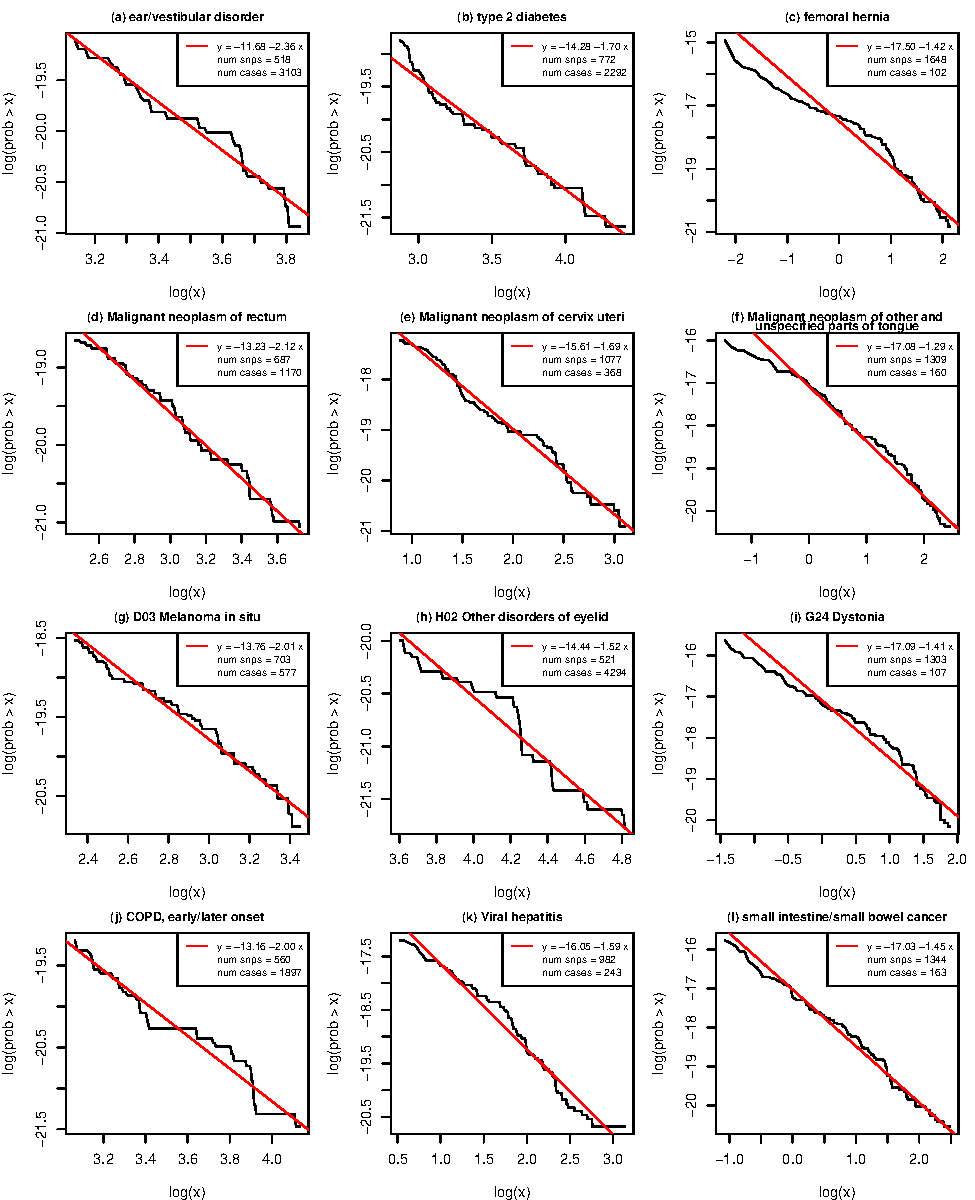
\includegraphics{snp_effects/examples}
    \end{center}
    \caption{
        TODO: cut this down to just 2 SNPs and move this figure to the supplement; change 'x' to 't' in axis labels.
        Tail distributions of frequency-weighted effects
        for twelve randomly chosen phenotypes.
        In each, for a phenotype with $N$ SNPs,
        effect sizes $e_i$ and frequencies $p_i$,
        the black line shows
        $\log \frac{1}{N} \sum_{i : |e_i| > t} p_i$ (vertical axis)
        against $\log t$ (horizontal axis);
        the red line shows the least-squares linear fit;
        each plot only covers the 10\% largest-effect SNPs.
        Legends show the coefficients of the red line; the slope on `x' is $\alpha$,
        the estimated exponent;
        ``num snps'' is the number of SNPs for the phenotype with $p$-value less than $10^{-8}$,
        and ``num cases'' is the reported number of the rougly 360,000 individuals
        recorded as having the listed phenotype.
        \label{fig:example_snps}
    }
\end{figure}

We applied this procedure to results from models fit on both sexes,
after removed phenotypes related to employment, drug treatments, and diet.
This left us with 1,108 phenotypes for which which could estimate the tail exponent.
For the main results,
we then restricted to phenotypes having non-missing numbers of ``cases'' and ``controls''
and a sample size of at least 300,000 (i.e., not more than 61,194 of 361,194 missing phenotypes).
We also removed
the 65 remaining phenotypes that are common (more than 10,000 cases),
as these often showed very different patterns
(e.g., effect size distributions).
This left us with 695 phenotypes;
plots including the 413 ``filtered'' phenotypes are provided in
Supplementary Figure~\ref{sfig:unfiltered_hist}.

Resulting values of the tail exponent $\alpha$ are shown in Figure~\ref{fig:exponent_hist}.
Estimated tail exponents range from about 1 to 2.5,
and 28.9\% had estimated values less than 1.5.
A concern could be that ``noisier'' phenotypes,
for which estimated effect sizes are less reliable,
might lead to larger estimated tail exponents;
for this reasons, we looked for an association between
tail exponent and two proxies for power,
number of SNPs (i.e., number of SNPs with $p$-value less than $10^{-8}$)
and number of cases.
Interestingly, the result in nonmonotonic,
with exponents closer to $\alpha=2$ for phenotypes with around 1000 cases,
and lower exponents for rarer \emph{and} more common phenotypes.
(A similar pattern is seen for ``number of SNPs'',
but this may be due to association with number of cases.)
This may indicate a statistical artifact,
or it may be a result of biological differences in genetic architecture
between more and less common phenotypes.

\begin{figure}
    \begin{center}
    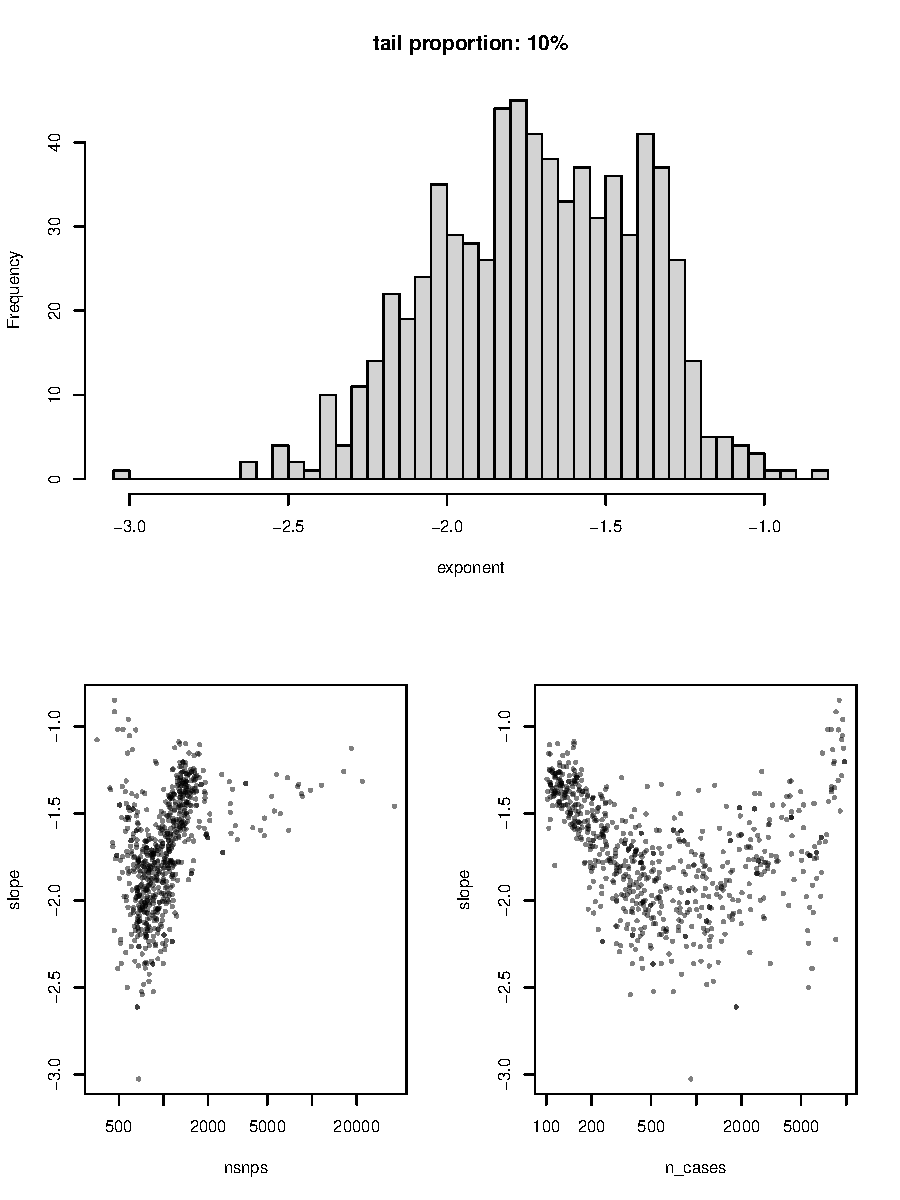
\includegraphics{snp_effects/results_10}
    \end{center}
    \caption{
        Estimated values of the tail exponent, $\alpha$,
        for 775 illness-related binary phenotypes:
        \textbf{(A)} distribution of values; and plotted against
        \textbf{(B)} number of SNPs, and
        \textbf{(C)} number of cases.
        \label{fig:exponent_hist}
    }
\end{figure}


%%%%%%%%%%%%%%%%%%%%%%
\section{Extending the infinitesimal model}  % TODD

\comment{Copied from \texttt{eugene\_notes.tex}:}

Let $X$ be a population of size $N$, recorded as the empirical distribution on phenotypes
\begin{align*}
    X = \frac{1}{N} \sum_{i=1}^N \delta_{x_i} .
\end{align*}
This evolves as a Moran process under the infinitesimal model
with death rates depending on state $x$.
Concretely, an individual whose phenotype is $x$
dies at rate $1 + \mu(x)$
and is replaced by a new individual of phenotype
\begin{align*}
  \frac{y + z}{2} + \xi ,
\end{align*}
where $y$ and $z$ are independent draws from $X$
and $\xi$ is an independent $N(0, \eta^2)$.
Let $\nu(X)$ denote the distribution of $\frac{y + z}{2} + \xi$.
This has generator
\begin{align*}
    \mL \Phi(X)
    &=
    \int \int \int \int
    \left( \Phi(X + \frac{1}{N} \delta_{(y+z)/2 + \xi} - \frac{1}{N} \delta_x) - \Phi(X) \right)
    (1 + \mu(x)) X(dx) X(dy) X(dz) e^{-(\xi/\eta)^2/2} d\xi \\
    &=
    \int \int
    \left( \Phi(X + \frac{1}{N} \delta_u - \frac{1}{N} \delta_x) - \Phi(X) \right)
    (1 + \mu(x)) X(dx) \nu(X)(du) .
\end{align*}

For a test function $\phi$, setting $\Phi(X) = \ip{\phi}{X}$
we get the first moment
\begin{align*}
    \mL \ip{\phi}{X}
    &=
    \frac{1}{N} \int \int \int \int
    \left( \phi \left( \frac{y+z}{2} + \xi \right)
         - \phi(x) \right)
    (1 + \mu(x)) X(dx) X(dy) X(dz) e^{-(\xi/\eta)^2/2} d\xi  \\
    &=
    \frac{1}{N} \ip{\phi}{\nu(X)}\ip{1+\mu}{X}
    - \frac{1}{N} \ip{\phi}{(1+\mu) X} .
\end{align*}
Note that $\ip{\phi}{\partial_{\nu(X)} X} = \ip{\phi}{\nu(X)}$,
so that this is a first derivative in the direction of
$\ip{1+\mu}{X} \nu(X) - (1+\mu) X$.

More generally, if $\Phi(X) = \prod_i \ip{\phi_i}{X}$ then
\begin{align*}
    \mL \Phi(X)
    &=
    \frac{1}{N} \sum_i \left( 
        \ip{1+\mu}{X} \ip{\phi_i}{\nu(X)}  - \ip{\phi_i}{(1+\mu)X}
    \right)
    \prod_{j \neq i} \ip{\phi_j}{X} 
    + O(1/N^2) .
\end{align*}
This implies that after rescaling time by $N$
and suitible other caveats,
the limiting process is a deterministic flow in the direction of 
$\nu(X) \ip{1+\mu}{X} - (1+\mu)X$.

\paragraph{Stable measures}
If $Z$ is a fixed point of this flow,
then $\nu(Z)\ip{1+\mu}{Z} = (1+\mu)Z$.
Any measure $Z$ that is a fixed point has the property that
(the average of two independent draws plus segregation noise)
is equal in distribution to
(a $1+\mu$-weighted draw).
Concretely, with $A$, $B$, and $C$ independent draws from $Z$,
$$\begin{aligned}
    \E\left[ f\left( \frac{A+B}{2} + \xi \right) \right]
    &=
    \frac{\E\left[ f(C) (1+\mu(C)) \right]}{\E[1+\mu(C)]} .
\end{aligned}$$

\comment{Copied from \texttt{MeanFlow.tex}:}

Assume that $Z$ is a finite measure, and without loss of generality normalized to have total mass one.

Throughout, I'll be using the characteristic function of $Z$, which I'll denote by 
\[
	\phi(\theta) = \mathbb{E}\left[e^{i\theta Z}\right],
\]
and the characteristic function of $\xi$, $\Phi(\theta)$.

\section{No Selection}

First, consider the case without selection, so $\mu$ is a constant.  Then, our condition on the characteristic function simplifies to
\begin{equation}\label{CHARACTERISTIC}
	{\textstyle \phi\left(\frac{\theta}{2}\right)^{2}} \Phi(\theta) %e^{-\frac{\eta^{2}\theta^{2}}{2}} 
	= \phi(\theta),
\end{equation}
\ie $\phi(\theta)$ is a fixed point of $F$, where
 \[
	F(\phi)(\theta) = {\textstyle \phi\left(\frac{\theta}{2}\right)^{2}} \Phi(\theta).
\]
In particular, we can characterize all possible fixed points by considering the iterates of an arbitrary characteristic function, $\varphi(\theta)$, for  any distribution on $\mathbb{R}$.  

Iterating $F$ $n$ times, we get
\[
	F^{(n)}(\varphi)(\theta)
	=  {\textstyle \varphi\left(\frac{\theta}{2^{n}}\right)^{2^{n}}}\prod_{k=1}^{n-1} {\textstyle \Phi\left(\frac{\theta}{2^{k}}\right)^{2^{k}}},
\]
so that
\[
	\phi(\theta) = \lim_{n \to \infty} \varphi\left(\frac{\theta}{2^{n}}\right)^{2^{n}}\prod_{k=1}^{n-1}\Phi\left(\frac{\theta}{2^{k}}\right)^{2^{k}}
\]
is a fixed point whenever this limit exists.  

Since $\varphi$ and $\Phi$ are characteristic functions, they are absolutely continuous and $\phi(0) = 1$, and thus non-zero in a neighbourhood of 0. In particular, $\psi(\theta) = \ln{\varphi}(\theta)$ and $\Psi(\theta) = \ln{\Phi(\theta)}$ exist in some neighbourhood of 0 as well.  From the above, we have
\[
	\ln{F^{(n)}(\varphi)(\theta)} = {\textstyle 2^{n} \psi\left(\frac{\theta}{2^{n}}\right)} 
		+ \sum_{k=1}^{n-1}  {\textstyle 2^{k} \Psi\left(\frac{\theta}{2^{k}}\right)}.
\]

\subsection{Noise Terms}

We now analyse the component arising from the noise $\xi$.  First, we consider the case when $\Psi(\theta)$ is twice continuously differentiable, so $\xi$ has finite mean $m = \Psi'(0)$ and variance $\eta^{2 = \Psi''(0)}$.   Taylor's theorem then tells us that for $\theta$ sufficiently small, 
\[
	\Psi(\theta) = m\theta + \frac{\eta^{2}}{2} \theta^{2} + r(\theta)\theta^{2},
\]
where $r(\theta) \to 0$ as $\theta \to 0$.  Then,
\begin{align*}
	 \sum_{k=1}^{n-1}  {\textstyle 2^{k} \Psi\left(\frac{\theta}{2^{k}}\right)}
	 &=  \sum_{k=1}^{n-1} 2^{k} {\textstyle \left(m \frac{\theta}{2^{k}} - \frac{\eta^{2}}{2}  \frac{\theta^{2}}{2^{2k}}
		+ r\left(\frac{\theta}{2^{k}}\right)\frac{\theta^{2}}{2^{2k}}\right)}\\
	&= (n-1) m - \eta^{2} \theta^{2} (1 - 2^{-n+1}) 
		+ \sum_{k=1}^{n-1} {\textstyle r\left(\frac{\theta}{2^{k}}\right)\frac{\theta^{2}}{2^{k}}}
 \end{align*}

Immediately, we see that for the limit to exist, we must have $m = 0$; if we assume that $r(\theta) \equiv 0$, so that the noise is $N(0,\eta^{2})$, then the limiting distribution is $N(0,2\eta^{2})$. We note that when  $r(\theta)$ is non-zero, we don't expect the higher order terms to vanish.

Now, consider the case when $\Psi(\theta)$ corresponds to a stable law, so
\[
	\Psi(\theta) = im\theta + c|\theta|^{\alpha} (1-i\beta \text{sgn}(\theta)\omega_{\alpha}(\theta))
\]
for $\alpha \in (0,2]$, $\beta \in [-1,1]$, $c \geq 0$, and $m \in \mathbb{R}$ and
\[
	\omega_{\alpha}(\theta) = \begin{cases}
		\tan{\frac{\pi\alpha}{2}} & \text{if $\alpha \neq 1$, and}\\
		-\frac{2}{\pi}\ln{|\theta|} & \text{if $\alpha = 1$.}
	\end{cases}
\]
We then have
\begin{multline*}
	 \sum_{k=1}^{n-1}  {\textstyle 2^{k} \Psi\left(\frac{\theta}{2^{k}}\right)}
	 =  \sum_{k=1}^{n-1} im\theta + 2^{(1-\alpha)k} c|\theta|^{\alpha} {\textstyle\left(1-i \beta\text{sgn}(\theta)\left(\frac{\theta}{2^{k}}\right)
	 	 \omega_{\alpha}\left(\frac{\theta}{2^{k}}\right)\right)}\\
	= 
	\begin{cases}
		 im(n-1)\theta + c|\theta|^{\alpha}\frac{1-2^{(1-\alpha)n}}{1-2^{1-\alpha}}\left(1-i\beta \text{sgn}(\theta) \tan{\frac{\pi\alpha}{2}}\right) & \text{if $\alpha \neq 1$, and}\\	
		 \begin{multlined}
		 im(n-1)\theta + c|\theta|^{\alpha}  \left(\frac{1-2^{(1-\alpha)n}}{1-2^{1-\alpha}}
		 \left(1+i \beta \text{sgn}(\theta)\frac{2}{\pi}\ln{|\theta|} \right)\right.\\
		\left. -i\beta \text{sgn}(\theta) \frac{2^{1-\alpha} + (n(2^{1-\alpha}-1)-1)2^{(1-\alpha)n})}{(1-2^{1-\alpha})^{2}}\frac{2}{\pi}\ln{2}
		\right)    
		\end{multlined}
		& \text{if $\alpha = 1$.}
	\end{cases}
\end{multline*}
This converges as $n \to \infty$ if and only if $m = 0$ and $\alpha > 1$, in which case the limit is 
\[
	 \frac{c}{1-2^{1-\alpha}}|\theta|^{\alpha}\left(1-i\beta \text{sgn}(\theta) \tan{\frac{\pi\alpha}{2}}\right), 
\]
which corresponds to a $\left(\alpha,\beta, \frac{c}{1-2^{1-\alpha}},0\right)$-stable law.

\subsection{Reproductive Terms}

We now consider the terms $2^{n} \psi\left(\frac{\theta}{2^{n}}\right)$, which we call the reproductive terms.  Proceeding as below, we consider the limit
%We note that this does not exclude the possibility of distributions without a mean; % \eg if $\eta =0$, then \eqref{CHARACTERISTIC} is satisfied by the family of Cauchy distributions with characteristic functions $\phi(\theta) = e^{i m \theta - \gamma |\theta|}$; one can check that these are the only stable laws satisfying \eqref{CHARACTERISTIC}.%  One can similarly exclude the stable laws without mean ($\alpha \leq 1$) by inspection in the case of $\eta > 0$. 
%Now, to exhaust all possibilities, observe that by iterating, we we also have that 
%\[
%	\psi(\theta) = 2^{n}\psi\left(\frac{\theta}{2^{n}}\right) 
%\]
%\ie we must have 
\[
		\alpha(\theta) = \lim_{n \to \infty} 2^{n}\psi\left(\frac{\theta}{2^{n}}\right).
\]
Because $\psi(\theta)$ is the logarithm characteristic function, it must be uniformly continuous and vanish at 0, and thus $\alpha(\theta)$ as well.  We also have that for all integers $k$, 
\[
	\alpha(2^{k} \theta) = \lim_{n \to \infty} 2^{n}\psi\left(\frac{2^{k} \theta}{2^{n}}\right) =  \lim_{n \to \infty} 2^{k} 2^{n-k} \psi\left(\frac{\theta}{2^{n-k}}\right) = 2^{k} \alpha(\theta).
\]
In particular, we see that given any continuous function $\alpha(\theta)$, $\theta \in [1,2]$, such that $\alpha(2) = 2\alpha(1)$, $\alpha$ is defined for all positive reals.  We can extend the definition to the negative reals via the Hermitian property for $\phi(\theta)$: $\phi(-\theta) = \overline{\phi(\theta)}$ implies that $\alpha(-\theta) = \overline{\alpha(\theta)}$. 

Now, from the above, 
\[
	\frac{\alpha(\theta)}{\theta} = \frac{\alpha(2^{k} \theta)}{2^{k}\theta} \to \alpha'(0+),
\]
as $k \to - \infty$ if the latter exists (\ie there is a unique left-hand limit at zero).  In this case, setting $-\gamma + i m = \alpha'(0+)$, we have
\[
	\alpha(\theta) = \begin{cases} 
		i m\theta - \gamma \theta & \text{if $\theta \geq 0$, and}\\
		i m\theta + \gamma \theta & \text{if $\theta < 0$}.
	\end{cases}
\]
\ie if $\gamma > 0$, then $e^{\alpha(\theta)} = e^{im \theta -\gamma|\theta|}$ is the characteristic function of a Cauchy distribution and $\phi(\theta)$ is the characteristic function of the sum of Cauchy and Gaussian random variables, whereas if $\gamma = 0$, then $e^{\alpha(\theta)} = e^{im \theta}$ is the Fourier transform of a Dirac mass at $m$, so the limiting random variable is the Gaussian $N(m,\eta^{2})$. 

Finally, we remark that if $\frac{\alpha(\theta)}{\theta}$ is non-constant for $\theta > 0$, then $\alpha'(0+)$ does not exist. 

\subsection{Other Solutions?}

We would naturally like to know if these two exhaust the possible solutions.  To this end, we recall Bochner's theorem, which tells us that a function $\phi(\theta)$ is the characteristic function of a random variable if and only if
\begin{enumerate}[(i)]
\item $\phi(\theta)$ is uniformly continuous,
\item $\phi(0) = 1$,
\item $\phi(-\theta) = \overline{\phi(\theta)}$, and
\item $\phi(\theta)$ is \textit{positive definite}: for all $n$ and all $\theta_{1},\ldots,\theta_{n} \in \mathbb{R}$, the matrix with entries
\[
	a_{ij} = \phi(\theta_{i}-\theta_{j})
\]
is positive definite.
\end{enumerate}
Given $\alpha(\theta)$ as above, the corresponding function $\phi(\theta) = e^{\alpha(\theta)-\eta^{2}\theta^{2}}$ 
or $\phi(\theta) = e^{\alpha(\theta) - \frac{c}{1-2^{1-\alpha}}|\theta|^{\alpha}\left(1-i\beta \text{sgn}(\theta) \tan{\frac{\pi\alpha}{2}}\right)}$ satisfies the first three criteria.  We will now seek to identify which $\alpha(\theta)$ result in positive definite $\phi(\theta)$.  When $\alpha(\theta) = im \theta -\gamma|\theta|$ for $\gamma > 0$, this is immediate, as $e^{\alpha(\theta)}$ is then the characteristic function of a Cauchy random variable.

We can also easily exclude the case $\gamma < 0$ using a simple consequence of positive definiteness in the case when $n=2$ (name criterion): if $\phi(\theta)$ is positive definite, then $|\phi(\theta)| \leq 1$.  For us, this requires that 
\[
	\Re \alpha(\theta) \leq  \eta^{2} \theta^{2},\; resp. \; < \frac{c}{1-2^{1-\alpha}}|\theta|^{\alpha}
\]
which is violated for small values of $\theta$ when $\gamma < 0$ (recall $\alpha > 1$). 

\noindent\emph{Question:} how can we use positive definiteness to exclude $\alpha(\theta)$ with $\Re \alpha(\theta) \leq  \eta^{2} \theta^{2}$ so that $\alpha'(0+)$ does not exist?

\begin{rem}
Polya has shown that if $\phi(\theta)$ is convex and satisfies the first three criteria of Bochner's theorem, then $\phi(\theta)$ is a characteristic function.  In our case, if $\alpha(\theta)$ is convex, then $e^{\alpha(\theta)}$ is as well; a proof-by-picture, however, shows that the only choice of $\alpha(\theta)$ that is convex (or concave, for that matter) for $\theta > 0$ is a linear function, so Polya's criterion doesn't give us any new characteristic functions.
\end{rem}


\subsection{Stabilizing Selection}
    \label{sec:stabilizing_selection}

\subsubsection{Gaussian Solution}
    \label{sec:stabilizing_gaussian}

Now, consider the case when $1+ \mu(x) = e^{a x^{2}}$.  In this case there is a Gaussian solution: suppose $Z$ is Gaussian with mean $m$ and variance $\sigma^{2}$.  Then,
\[
	\phi(\theta) = e^{i m \theta - \frac{1}{2} \sigma^{2} \theta^{2}}.
\]
Moreover, provided $a < \frac{1}{2\sigma^{2}}$, we can explicitly compute $\frac{\mathbb{E}\left[e^{i \theta Z}(1+\mu(Z))\right]}{\mathbb{E}[1+\mu(Z)]}$  to conclude that
if $\xi$ is Gaussian with mean zero and variance $\eta^2$,
then equation~\eqref{CHARACTERISTIC} is
\comment{something not right here? need a factor of 2 on the left?}
\[
	e^{i m \theta - \frac{1}{2} \left(\frac{\sigma^{2}}{2} + \eta^{2}\right)\theta^{2}}
	= e^{i \frac{m}{1-2 a \sigma^{2}}\theta 
		- \frac{1}{2} \frac{\sigma^{2}}{1-2 a \sigma^{2}}\theta^{2}},
\]
which, equating real and complex components, has a solution provided $m = 0$ and
\[
	\sigma^{2} = \frac{\sqrt{16 a^{2} \eta^{4} + 24 a \eta^{2}+1} - 4a \eta^{2} -1}{4a} 
	=  2\eta^{2}(1-4a\eta^{2}) + O(a^{2}).
\]

\subsubsection{Cauchy Solution}
    \label{sec:stabilizing_cauchy}

In the case of a Cauchy random variable, we again have an explicit expression for the probability distribution, which, proceeding as above, allows us to construct an explicit solution when $1+ \mu(x) = \frac{\delta^{2}}{\gamma^{2}} \frac{\gamma^{2} + x^{2}}{\delta^{2} + x^{2}}$ for $\delta > \gamma > 0$ and the noise $\xi$ is given by a $\text{Cauchy}(0,\delta-\gamma)$ random variable (\ie corresponding to a stable $(0,0,\delta-\gamma,0)$ law).

If we now suppose that $Z$ is a $\text{Cauchy}(0,\gamma)$ random variable.  Then $Z$ has probability density function $\frac{\gamma}{\pi} \frac{1}{\gamma^{2} + x^{2}}$, whereas 
\[
	\frac{\mathbb{E}\left[e^{i \theta Z}(1+\mu(Z))\right]}{\mathbb{E}[1+\mu(Z)]}
	= e^{-\delta |\theta|} = e^{-2\gamma \left|\frac{\theta}{2}\right|-(\delta-\gamma)|\theta|}
\]
which we recognize as being equal to $\phi\left(\frac{\theta}{2}\right)^{2} \Phi(\theta)$,
and so solves equation~\eqref{CHARACTERISTIC}.

%(here, see a saturating cost to being away from the optimal phenotype $x = 0$: the mortality is maximized at  $\frac{\beta^{2}}{\alpha^{2}}$.

\bigskip

\noindent\emph{Question:} other stable laws?


%%%%%%%%%%%%%%%%%%%%%%
\section{Convergence to the non-infinitesimal model}  % TODD

%%%%%%%%%%%%%%%%%%%%%%
\section{Stationary distributions}  % TODD

%%%%%%%%%%%%%%%%%%%%%%
\section{Simulations}  % PETER

In Section~\ref{sec:stabilizing_selection}
we have found two explicit conditions in which
if the form of segregation noise and stabilizing selection
satisfy certain conditions,
then the limiting phenotype distribution
will be either Gaussian (Subsection~\ref{sec:stabilizing_gaussian}
or Cauchy (Subsection~\ref{sec:stabilizing_cauchy}.
Furthermore, we expect based on
\citet{barton2017infinitesimal} and arguments above
that the distribution of segreation noise
is determined by the tail exponent of the distribution of effect sizes
(under appropriate assumptions; e.g., that most mutations are of small effect).
However, it is not clear how selection would affect these arguments,
especially in the stable case where some number of mutations are expected to
\emph{not} have small effect (and therefore such mutations will not be nearly neutral).

Therefore,
to study how this works in practice, we turn to simulation.
We used SLiM v3 \comment{(cite)}
to simulate a discrete-time approximation to the continuous-time Moran model described above
as follows.
Individuals are diploid and sexual;
the genome is of lenth $10^8$bp with a uniform recombination rate of $10^{-8}$ crossovers per bp;
mutations occur at a rate of $m$ per bp.
Each new mutation is independently assigned an ``effect''
drawn from the ``effect size distribution'' (and will be either Gaussian or Cauchy).
The phenotype of each individual is determined additively
by summing the effects of all mutations they carry across both chromosomes.
Let $f(z) = 1 + \mu(z)$
be the ``fitness'' of an individual with phenotype $z$,
and let $dt$ be a small constant (we took $dt=0.01$).
Then, at each time step
each individual dies with probability $1 - \exp(-dt f(z))$;
if there are $k$ such individuals chosen to die in a given time step,
then we choose $k$ individuals uniformly and without replacement
to produce new offspring;
for each such reproduction event the parent chooses a mate uniformly at random from the population.
This maintains the population at a fixed size, $N$.
(Note that individuals may self and individuals chosen to die may also reproduce,
but in a large population these details should be unimportant.)

We compared two situations:
(1) the effect size distribution was Gaussian with mean zero and standard deviation $\sigma_g$,
and $f(z) = e^{\alpha z^2}$; and
(2) the effect size distribution was Cauchy, centered at zero and with width $\delta - \gamma$
and $f(z) = (\delta/\gamma) (\gamma + z^2) / (\delta + z^2)$.
\comment{TODO: just refer to equations above?}
We ran simulations of each with $N=XXX$ for XXX time steps of ``burn-in''
(judged to be long enough as the number of segregating mutations had plateaued),
following which we recorded the phenotypes of each new offspring and their two parents
for XXX time steps (a total of around YYY offspring).

Figure XXX shows the resulting distributions of segregation noise:
i.e., the distribution of child phenotype minus average of parents' phenotypes,
across all offspring following burn-in.


\bibliographystyle{plainnat}
\bibliography{refs}

\appendix

\begin{figure}
    \begin{center}
    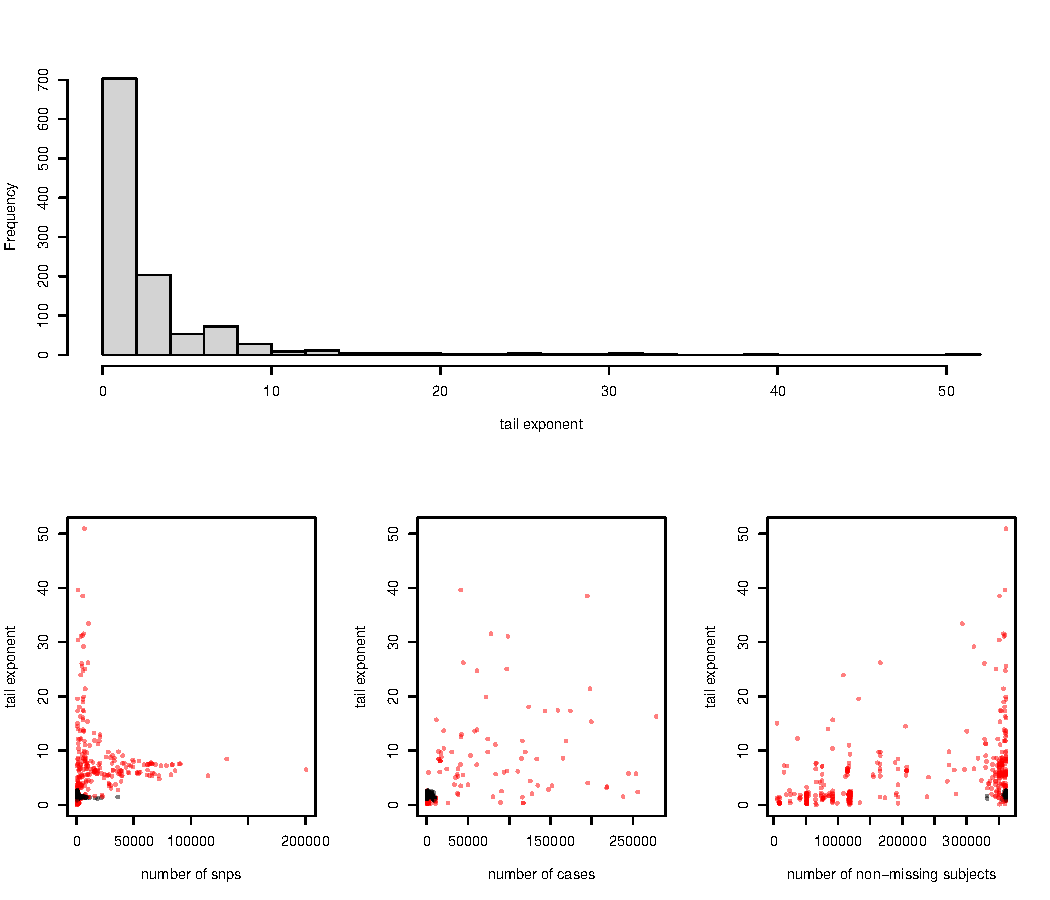
\includegraphics{snp_effects/unfiltered_results_10}
    \end{center}
    \caption{
        Estimated values of the tail exponent, $\alpha$,
        for 1108 illness-related binary phenotypes,
        including the 333 phenotypes removed in filtering,
        which are shown as red points in lower plots.
        \textbf{(A)} distribution of values; and plotted against
        \textbf{(B)} number of SNPs,
        \textbf{(C)} number of cases, and
        \textbf{(C)} number of non-missing subjects.
        \label{fig:unfiltered_hist}
    }
\end{figure}

\end{document}
